\documentclass[a4paper,12pt,fleqn]{article}
\usepackage{amsmath, amssymb}
\usepackage{bbm}
\usepackage{enumitem}
\usepackage{array}
\usepackage{fancyhdr}
\usepackage{graphicx}

% Insert your course information here %%%%%%%%%%%%%%%%%%%%%%%%%%%%%%%%%%

\newcommand{\titlehd}{Computational Data Analysis}
\newcommand{\examtype}{\bf Final Exam}
\newcommand{\examdate}{Due Dec. 13, 2019}
\newcommand{\examcode}{ISYE 6740}
%\newcommand{\writetime}{}
\newcommand{\total}{100}
\newcommand{\lastwords}{End of Examination}

%%%%%%%%%%%%%%%%%%%%%%%%%%%%%%%%%%%%%%%%%%%%%%%%%%%%

%\setcounter{MaxMatrixCols}{10}
\newtheorem{theorem}{Theorem}
\newtheorem{acknowledgement}[theorem]{Acknowledgement}
\newtheorem{algorithm}[theorem]{Algorithm}
\newtheorem{axiom}[theorem]{Axiom}
\newtheorem{case}[theorem]{Case}
\newtheorem{claim}[theorem]{Claim}
\newtheorem{conclusion}[theorem]{Conclusion}
\newtheorem{condition}[theorem]{Condition}
\newtheorem{conjecture}[theorem]{Conjecture}
\newtheorem{corollary}[theorem]{Corollary}
\newtheorem{criterion}[theorem]{Criterion}
\newtheorem{definition}[theorem]{Definition}
\newtheorem{example}[theorem]{Example}
\newtheorem{exercise}[theorem]{Exercise}
\newtheorem{lemma}[theorem]{Lemma}
\newtheorem{notation}[theorem]{Notation}
\newtheorem{problem}[theorem]{Problem}
\newtheorem{proposition}[theorem]{Proposition}
\newtheorem{remark}[theorem]{Remark}
\newtheorem{solution}[theorem]{Solution}
\newtheorem{summary}[theorem]{Summary}
\newenvironment{proof}[1][Proof]{\noindent\textbf{#1.} }{\ \rule{0.5em}{0.5em}}
\newcounter{questionnumber}
\stepcounter{questionnumber}

\newcommand{\questionnumber}{\noindent \arabic{questionnumber}\stepcounter{questionnumber})~~}
\newcommand{\truefalse}[1]{\questionnumber #1\\True~~~~~~~~False\\Explanation if False:\\ \vspace{3cm}}
\newcommand{\norm}[1]{\|#1\|}
\newcommand{\RR}{\mathbb{R}}
\newcommand{\argmin}{\mathop{\arg\min}}

% ANU Exams Office mandated margins and footer style
\setlength{\topmargin}{0cm}
\setlength{\textheight}{9.25in}
\setlength{\oddsidemargin}{0.0in}
\setlength{\evensidemargin}{0.0in}
\setlength{\textwidth}{16cm}
\pagestyle{fancy}
\lhead{} 
\chead{} 
\rhead{} 
\lfoot{} 
\cfoot{\footnotesize{Page \thepage \ of \pageref{finalpage} -- \titlehd \ (\examcode)}} 
\rfoot{} 

% DEPRECATED: ANU Exams Office mandated margins and footer style
%\setlength{\topmargin}{0cm}
%\setlength{\textheight}{9.25in}
%\setlength{\oddsidemargin}{0.0in}
%\setlength{\evensidemargin}{0.0in}
%\setlength{\textwidth}{16cm}
%\pagestyle{fancy}
%\lhead{} %left of the header
%\chead{} %center of the header
%\rhead{} %right of the header
%\lfoot{} %left of the footer
%\cfoot{} %center of the footer
%\rfoot{Page \ \thepage \ of \ \pageref{finalpage} \\
%       \texttt{\examcode}} %Print the page number in the right footer

\renewcommand{\headrulewidth}{0pt} %Do not print a rule below the header
\renewcommand{\footrulewidth}{0pt}


\begin{document}

% Title page
\begin{center}
\large\textbf{\titlehd}
\end{center}

\begin{center}
\large\textbf{\examcode}
\end{center}

\begin{center}
\textit{ \examtype -- \examdate}
\end{center}

%\begin{center}
%\textit{Writing Time: \writetime}
%\end{center}

\begin{center}
\textit{Total Score: \total}
\end{center}

\vspace{2cm}
If you think a question is unclear or multiple answers are reasonable, please write a brief explanation of your answer,
 to be safe. Also, show your work if you want wrong answers to have a chance at some credit: it lets us see how much you understood.\\\\
(Please sign the honor code below.) I have neither given nor received any unauthorized aid on this exam. I understand that the work contained herein is wholly my own without the aim from a 3rd person. I understand that violation of these rules, including using an authorized aid or copying from another person,
may result in my receiving a 0 on this exam .
\begin{table}[h]
\centering
\begin{tabular}{m{8cm}}
\\
\\
\vspace{0.2in}
\textbf{Name}: 
\vspace{0.7in}

\textbf{GT ID:}
\vspace{0.7in}


\textbf{GT Account:}
\end{tabular}
\end{table}
\newpage

\begin{table}[h]
\centering
\begin{tabular}{| m{6cm} | m{6cm} |}
\hline
\vspace{0.5cm}
Question 1 [15 points] & \\
\vspace{0.5cm} &\vspace{0.5cm}\\
\hline
\vspace{0.5cm}
Question 2 [15 points] & \\
\vspace{0.5cm} &\vspace{0.5cm}\\
\hline
\vspace{0.5cm}
Question 3 [15 points] & \\
\vspace{0.5cm} &\vspace{0.5cm}\\
\hline
\vspace{0.5cm}
Question 4 [20 points] &  \\
\vspace{0.5cm} &\vspace{0.5cm}\\
\hline
\vspace{0.5cm}
Question 5 [10 points] & \\
\vspace{0.5cm} &\vspace{0.5cm}\\\hline
\vspace{0.5cm}
Question 6 [25 points] & \\
\vspace{0.5cm} &\vspace{0.5cm}\\\hline

\hline
\end{tabular}
\end{table}


% End title page

%
%\newpage
%
%\section{K-means}
%\questionnumber{
%
%Given data points $x_1,x_2,\ldots,x_n \in \mathbb{R}^d$. We can modify K-means objective with $\ell_1$ regularization. More specifically, we consider
%\[
%\argmin_{S=\{S_1,\ldots,S_k\}} \sum_{j=1}^{k}\sum_{x_i\in S_j}\|x_i-\mu_j\|^2_2 + \lambda \sum_{j=1}^{k}\|\mu_j\|_1
%\]
%where $\lambda > 0$ is the regularization parameter.
%where $\mu_j$ is the mean of points in $S_j$. 
%
%\begin{enumerate}
%	
%	\item[(a)]  Please describe the new 2-steps optimization for this problem. Are they different from the original problem?
%	
%	(Hint: you may need the fact that,$$\hat v = \argmin_v \frac{1}{2}\|u-v\|^2_2+\lambda \|v\|_1$$ has closed form solution $\hat{v}  = [\hat{v}_j]_{j=1}^d = [\mathrm{sign}(u_j)\max\{|u_j|-\lambda,0\}_{j=1}^d].$)
%	
%	\vspace*{160pt}
%	
%	\item[(b)] The $\ell_1$ regularization encourages sparsity of $\mu_j$ . If the results have the $m$-th entries of all $\mu_j$'s equal to zero, what will this imply?
%	\vspace*{80pt}
%	
%	\item[(c)] Let $\gamma_k$ and $\gamma'_k$ denote the global optimal objective value of k-means with and without $\ell_1$ regularization. Please compare $\gamma_k$ and $\gamma'_k$ ($<,\leq,\geq,=$) and prove this relation.
%	\vspace*{80pt}
%\end{enumerate}
%
%}
%
%\newpage
%
%\section*{Question 2. Spectral Clustering}
%Recall that spectral clustering is a method finding $K$ clusters on a graph/network $\mathcal{G}=(\mathcal{V},\mathcal{E})$, where $\mathcal{V} = \{1,\ldots,n\}$ is the $\mathcal{E}$ is the edge set. $w_{ij}$ is the weight of edge $e=(i,j) \in \mathcal{E} $. A cluster is a subset of vertexes, i.e. $\mathcal{G}_k \subseteq \mathcal{V},\; k=1,\ldots,K$. We define two useful quantities on two subsets of vertexes, $A$ and $B$: 
%\[cut(A,B)=\sum_{i\in A,j\in B}w_{ij}
%\quad \text{and} \quad
%assoc(A) = cut(A,\mathcal{V})=\sum_{i\in A,j\in \mathcal{V}}w_{ij}
%\]
%Thus we can define cut cost function to evaluate the quality of clustering, $$R^C(\mathcal{G}_1,\ldots,\mathcal{G}_K)=\sum_{k=1}^{K}cut(\mathcal{G}_k,\mathcal{V} \backslash \mathcal{G}_k)$$
% and the normalized cut cost function
% $$R^{NC}(\mathcal{G}_1,\ldots,\mathcal{G}_K)=\sum_{k=1}^{K}\frac{cut(\mathcal{G}_k,\mathcal{V} \backslash \mathcal{G}_k)}{assoc(\mathcal{G}_k)}$$
% 
% \begin{enumerate}
% 	
% 	\item[(a)]  Please explain the intuition behind $cut(A,B),assoc(A),R^C,R^{NC}$
% 	
% 	
% 	\newpage
% 	For simplicity, in the following questions we only consider $K=2$
% 	
%% 	\item[(b)] Show that minimizing $R^{NC}(\mathcal{G}_1, \mathcal{G}_2)$ has the following formulation:
%% 	$$ \min R^{C}(\mathcal{G}_1, \mathcal{G}_2) = \min f^TLf , \quad 
%% 	\text{where}\ f_i=  
%% 	\left\{ \begin{aligned}
%% 	1, i\in \mathcal{G}_1\\
%% 	-1, i\in \mathcal{G}_2
%% 	\end{aligned}
%% 	\right.
%% 	$$
%% 	Recall that the graph Laplacians was defined as $L=D-W$, where $$D=diag(\sum_{j=1}^{n}w_{1j},\sum_{j=1}^{n}w_{2j},\ldots,\sum_{j=1}^{n}w_{nj})$$
%% 	
%% 	\item[(c)] We can we consider the relaxation of the above problem, i.e.,
%% 	 $$\min R^{C}(\mathcal{G}_1, \mathcal{G}_2) = \min f^TLf, \quad \text{subject to} \quad f^\top f = 1,$$ where the constraint is used to control the scale of $f$. Show that the solution of such problem is the eigen vector we used in the 
% 	
% 	\item[(b)] Show that minimizing $R^{NC}(\mathcal{G}_1, \mathcal{G}_2)$ has the following formulation:
% 	\begin{align} \min R^{NC}(\mathcal{G}_1, \mathcal{G}_2) = \min \frac{f^TLf}{f^TDf} , \quad 
% 	\text{where}\ f_i=  
% 	\left\{ \begin{aligned}
% 	\frac{1}{assoc(\mathcal{G}_1)}, i\in \mathcal{G}_1\\
% 	-\frac{1}{assoc(\mathcal{G}_2)}, i\in \mathcal{G}_2
% 	\end{aligned}
% 	\right. \label{eq:2.b}
% 	\end{align}
% 	Recall that the graph Laplacians was defined as $L=D-W$, where $$D=diag(\sum_{j=1}^{n}w_{1j},\sum_{j=1}^{n}w_{2j},\ldots,\sum_{j=1}^{n}w_{nj})$$
% 	
% 	\newpage
% 	\item[(c)] Next we consider the relaxation of the above problem, i.e.,
% 	\begin{align}\min R^{NC}(\mathcal{G}_1, \mathcal{G}_2) = \min \frac{f^TLf}{f^TDf}, \quad \text{subject to} \quad f^\top D\mathbf{1} = 0,\label{eq:2.c}
% 	\end{align}
% 	 Jusitify this is a relaxation of \eqref{eq:2.b}, i.e. for any solution of \eqref{eq:2.b} is a solution of \eqref{eq:2.c}
% 	
% 	\newpage
% 	\item[(d)] Show that the solution to \eqref{eq:2.c} is the eigen vector corresponding to second smallest eignevalue of the Graph Laplacian $L$. Just like the one we used in Spectral Clustering. (Noticing that the smallest eigenvalue is 0, and the corresponding eigen vector is $\mathbf{1}$) Here we can normalize $f$ for simplicity, i.e., you only need to consider the following problem
% 	 \begin{align}\min R^{NC}(\mathcal{G}_1, \mathcal{G}_2) = \min \frac{f^TLf}{f^TDf}=\min f^TLf, \notag \\ \text{subject to} \quad f^\top D\mathbf{1} = 0,\; f^TDf=1,\label{eq:2.d}
% 	\end{align} 
% 	where the additional constraint is only used for controlling the scale of $f$.
% 	\newpage
% 	
% \end{enumerate}

\clearpage
\section{Clustering [15 pts]}


\begin{enumerate}

\item (5 points) Explain what is the difference between $K$-means and spectral clustering? 

\vspace{1.5in}


\item (5 points) What is in common, and what is the main difference between spectral clustering and PCA?

\vspace{1.5in}

\item (5 points) For the following data (two moons), give one method that will successfully separate the two moons? Explain your rationale. 

\begin{center}
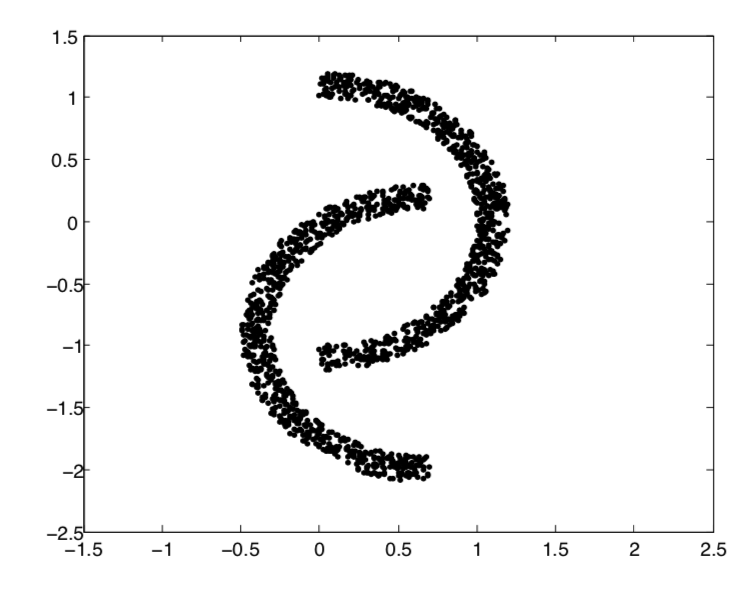
\includegraphics[width = 0.5\textwidth]{moon}
\end{center}

\end{enumerate}

\clearpage
\section{Classification [15 points]}

\begin{enumerate}
\item (5 points) List all methods below which can be used for classification:

(a) AdaBoost (b) Decision Trees (c) EM and Gaussian Mixture (d) Histogram (e) $K$-nearest neighbors (f) $K$-means (g) Kernel density estimation 
(h) Linear Regression (i) Logistic Regression (j) Naive Bayes. 



\vspace{1.3in}

\item (5 points) Which of the decision boundaries below correspond to (a) Random Forest, (b) Decision Tree, (c) SVM. Explain your reasons  to fully justify your answers. 
%
\begin{center}
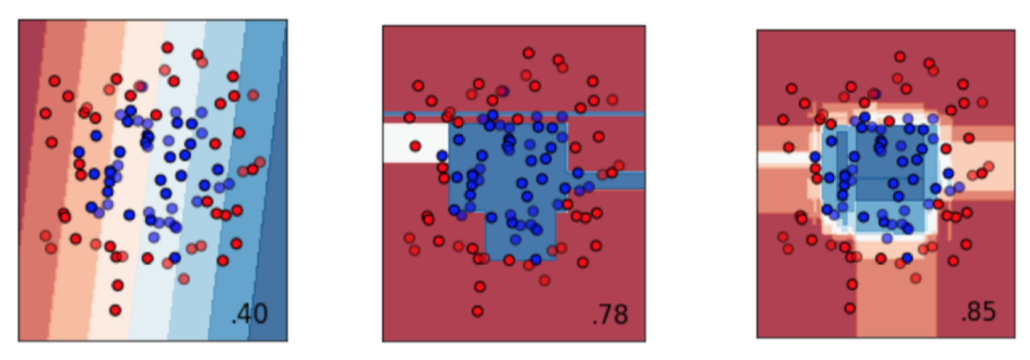
\includegraphics[width = 0.6\textwidth]{decision}
\end{center}

\vspace{1in}

\item (5 points) Is the following statement true / false: ``In the AdaBoost algorithm, the weights on all the
misclassified points will go up by the same multiplicative factor.'' Explain your reason.

\end{enumerate}


\clearpage
\section{SVM [15 points]}

Suppose we only have four training examples in two dimensions as shown in Fig. The positive samples at $x_1 = (0, 0)$, $x_2 = (2, 2)$ and negative samples at $x_3 = (h, 1)$ and $x_4 = (0, 3)$. 
%
\begin{center}
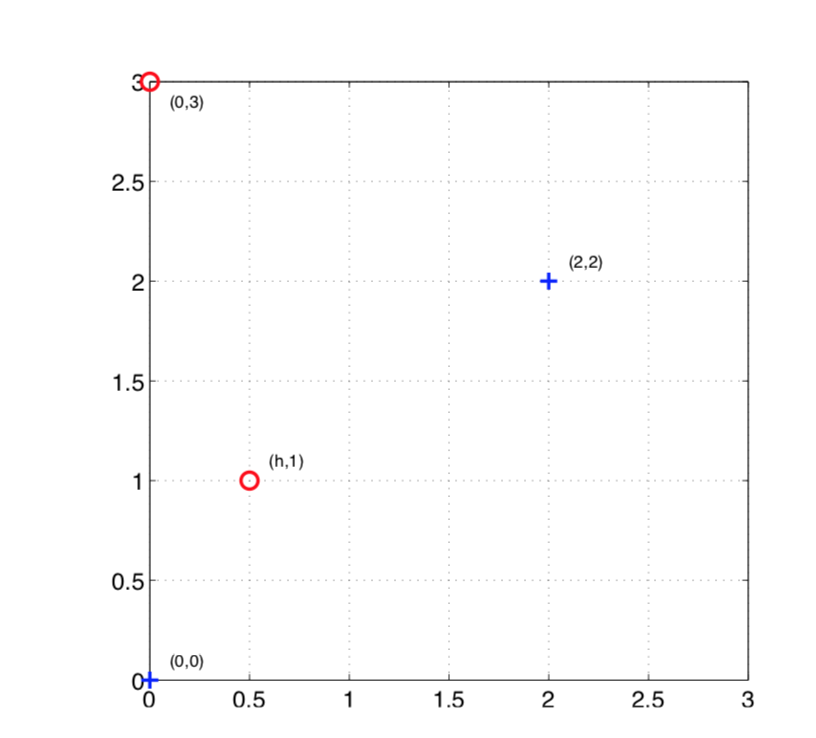
\includegraphics[width = 0.5\textwidth]{svm}
\end{center}

\begin{enumerate}
\item (5 points) For what $h$ s.t. $h > 0$ to be so that the training points are still linearly separable?

\vspace{1in}

\item (5 points) Does the orientation of the maximum margin decision boundary change as a function of $h$ when the points are separable?

\vspace{1.5in}

\item (5 points) Explain why only the data points on the ``margin'' will contribute to the decision boundary?
\end{enumerate}

\clearpage

\section{Variable section [20 points]}

Suppose we have data $\{x_i, y_i\}$, $i = 1, \ldots, m$, where $x_i \in \mathbb R^p$ corresponds to $p$ features.


\begin{enumerate}
\item (5 points) Write down the optimization problem we solve with Ridge Regression and Lasso. Make sure you explain your notations: which are the decision variables, and which are data. 

\vspace{1.5in}


\item (5 points) Which of the solution paths below corresponds to Ridge regression and which corresponds to Lasso?
%
\begin{center}
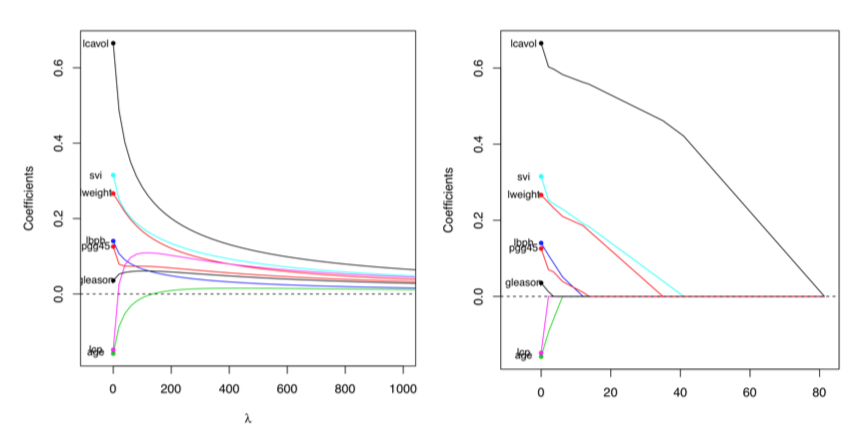
\includegraphics[width = 0.6\textwidth]{path}
\end{center}

\vspace{0.6in}

\item (5 points) Explain what's the difference between Lasso and Ridge regression. We need Lasso for what setting?

\vspace{0.9in}

\item (5 points) Explain how to tune the regularization parameters for Lasso and Ridge regression. 

\vspace{1.5in}

\end{enumerate}


\clearpage

\section{Neural networks [10 points].}

\begin{enumerate}
\item (5 points)
Consider a neural networks for a binary classification using sigmoid function for each unit. If the network has no hidden layer, explain why the model is equivalent to logistic regression. 
\item (5 points) 
Consider a simple two-layer network in the lecture slides. Given $m$ training data $(x^i, y^i)$, $i = 1, \ldots, m$, the cost function used to training the neural networks
\[
\ell(w, \alpha, \beta) = \sum_{i=1}^m (y^i - \sigma(w^T z^i))^2
\]
where $\sigma (x) = 1/(1+e^{-x})$ is the sigmoid function, $z^i$ is a two-dimensional vector such that  $z_1^i = \sigma(\alpha^T x^i)$, and $z_2^i = \sigma(\beta^T x^i)$. Show the that the gradient is given by
\[
\frac{\partial \ell(w, \alpha, \beta) }{\partial w}
= \sum_{i=1}^m 2(y^i - \sigma(u^i))\sigma(u^i)(1-\sigma(u^i)) z^i,
\]
where $u^i = w^T z^i$. Also find the gradient of $\ell(w, \alpha, \beta)$ with respect to $\alpha$ and $\beta$ and write down their expression.
\end{enumerate}

\clearpage

\section{Programming: Bayes and KNN classifier [25 points]}


In this programming assignment, you are going to apply the Bayes Classifier to handwritten digits classification problem. Here, we use the binary 0/1 loss for binary classification, i.e., you will calculate the miss-classification rate as a performance metric.

To ease your implementation, we selected two categories from USPS dataset in \textsf{usps-2cls.mat} (or \textsf{usps-2cls.dat}, \textsf{usps-2cls.csv}).

\begin{enumerate}
\item (15 points)
Your first task is implementing the classifier by assuming the covariance matrices for two classes are a diagonal matrix $\Sigma_1$, $\Sigma_ 2$. 

Using slides from ``Classification I'', assuming $P(y=1) = P(y=-1)$ (i.e., the prior distribution for two classes are the same), using Bayes decision rule to write down the decision boundary. (Hint, it should be a quadratic decision boundary.)
%\begin{itemize}
%\item[(a)] Full matrix, i.e., $\Sigma_1 = \Sigma_2 = \Sigma$ and $\Sigma$ is a dense matrix, i.e., all entries can be non-zero; 
%\item[(b)] Diagonal matrix, $\Sigma_1 = \Sigma_ 2 = D$, where $D$ is a diagonal matrix and 
%\item[(c)] Spherical (the diagonal has a constant value), $\Sigma_1 = \Sigma_ 2 = \sigma^2 I$. 
%\end{itemize}

Now we will estimate the mean vector and the sample covariance matrices for two classes using the training data (hint: you can use sample mean and sample covariance vector). Report the misclassification rate (error rate) over the training set and over the testing set averaged over the 100 random train/test splits by using different value of splitting ratio $p$. Explain and compare the performance of each classifier.

After implementing these methods, you should evaluate your algorithm on the given set. Repeat 100 times: split the dataset into two parts randomly, use $p$ portion for training and the other $1 - p$ portion for testing. Let $p$ change from 0.1, 0.2, 0.5, 0.8, 0.9.

Please implement the algorithm {\bf from scratch} yourself. Make sure to provide code, results (required above) together with necessary explanations to your results. 

\item (10 points) Now repeat the classification again using $K$-nearest neighbors, for $K = 5, 10, 15, 30$.  Repeat 100 times: split the dataset into two parts randomly, use $p$ portion for training and the other $1 - p$ portion for testing. Let $p$ change from 0.1, 0.2, 0.5, 0.8, 0.9. Report the training error and testing error for each case.

For this part, you may use any package that you like.  Make sure to provide code, results (required above) together with necessary explanations to your results. 

\end{enumerate}


\label{finalpage}

\end{document}